% 2007 年四川卷理科第 11 题：三条平行直线 l_1、l_2、l_3 与正三角形 ABC。
% 来源 PDF：gaokaomath-src/普通高考/2007/2007四川理.pdf，SHA256 6f3287a6ec1c136fb7e457cb0264d069c44eb8ff58a81cc3598f9c8f1395cc2d
% 原页：2007四川理.pdf 第 1 页（A3 三栏）第 2 栏，书页码 409，图在第 11 题选项上方。
% 重绘依据：三条水平线自上而下为 l_1、l_2、l_3，l_1 l_2 间距与 l_2 l_3 间距按题设 1:2
%   （取 1.0 : 2.0）；A 在 l_1 上居右，B 在 l_2 上居左，C 在 l_3 上且水平位置介于
%   B、A 之间（与 A 相近）；AB 向右上倾斜、BC 向右下倾斜、CA 近乎陡直，三边均为实线。
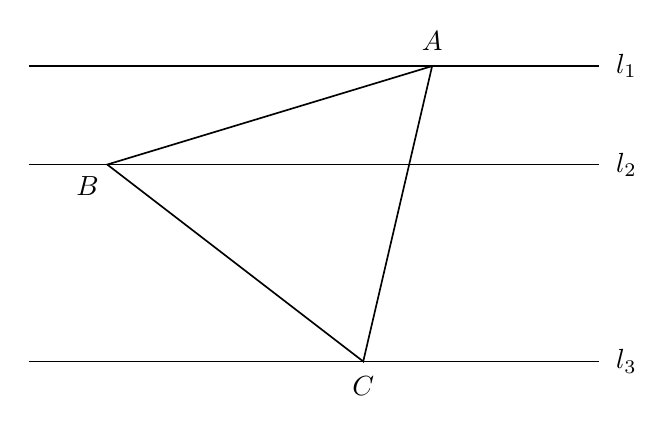
\begin{tikzpicture}[scale=1.25, semithick,
  every node/.style={inner sep=1.5pt}]
  % 三条平行线
  \draw (-0.2,2.2) -- (5.6,2.2);
  \draw (-0.2,1.2) -- (5.6,1.2);
  \draw (-0.2,-0.8) -- (5.6,-0.8);
  % 正三角形的三个顶点
  \coordinate (A) at (3.9,2.2);
  \coordinate (B) at (0.6,1.2);
  \coordinate (C) at (3.2,-0.8);
  \draw (A) -- (B) -- (C) -- cycle;
  \node[anchor=west] at (5.72,2.2) {$l_1$};
  \node[anchor=west] at (5.72,1.2) {$l_2$};
  \node[anchor=west] at (5.72,-0.8) {$l_3$};
  \node[anchor=south] at ([yshift=3pt]A) {$A$};
  \node[anchor=north east] at ([xshift=-1pt,yshift=-2pt]B) {$B$};
  \node[anchor=north] at ([yshift=-3pt]C) {$C$};
\end{tikzpicture}
